\chapter{Sequences and Convergence: The Foundation of Analysis}

\section{From Numbers to Processes}

\begin{intuition}
We've built the real numbers $\mathbb{R}$ with their completeness property. Now we study \textbf{infinite processes}:

\textbf{Question}: What does it mean for values to ``approach'' something?

\[\frac{1}{1}, \frac{1}{2}, \frac{1}{3}, \frac{1}{4}, \ldots \to 0\]

\[1, 1.4, 1.41, 1.414, 1.4142, \ldots \to \sqrt{2}\]

This chapter makes ``approaching'' and ``limit'' precise. These concepts underpin all of calculus and analysis.
\end{intuition}

\begin{historicalnote}
\textbf{The Birth of Rigor in Analysis}

\textbf{Ancient Greeks (c. 300 BCE)}:
\begin{itemize}
    \item Zeno's paradoxes: Achilles never catches the tortoise (infinite sums)
    \item Method of exhaustion: Approximating areas by polygons
    \item No formal notion of limit
\end{itemize}

\textbf{17th-18th Century (Calculus Era)}:
\begin{itemize}
    \item Newton (1665): Fluxions and infinitesimals
    \item Leibniz (1675): $dx$ and $dy$ as ``infinitely small quantities''
    \item Euler (1748): Manipulated infinite series freely
    \item \textbf{Problem}: No rigorous foundation---what \textit{is} an infinitesimal?
    \item Berkeley (1734): ``Ghosts of departed quantities''---criticized lack of rigor
\end{itemize}

\textbf{19th Century (Rigor Revolution)}:
\begin{itemize}
    \item \textbf{Bolzano (1817)}: First rigorous definition of continuity
    \item \textbf{Cauchy (1821)}: \textit{Cours d'Analyse}---sequences, limits, convergence
    \item \textbf{Weierstrass (1860s)}: $\epsilon$-$\delta$ definitions (``arithmetization of analysis'')
    \item \textbf{Dedekind (1872)}: Rigorous construction of $\mathbb{R}$
    \item Result: Calculus finally had solid foundations
\end{itemize}

Today, every analysis course begins with sequences and limits---the gateway to rigorous calculus.
\end{historicalnote}

\section{Sequences: Infinite Ordered Lists}

\begin{definition}[Sequence]
A \textbf{sequence} in $\mathbb{R}$ is a function $a: \mathbb{N}^+ \to \mathbb{R}$, where $\mathbb{N}^+ = \{1, 2, 3, \dots\}$.

We write $a(n)$ as $a_n$ and denote the sequence as:
\[(a_n)_{n=1}^\infty \quad \text{or} \quad (a_1, a_2, a_3, \ldots) \quad \text{or simply} \quad (a_n)\]

The value $a_n$ is called the \textbf{$n$-th term} of the sequence.
\end{definition}

\begin{convention}[Indexing]
While our natural numbers $\mathbb{N}$ start at 0, it is standard in analysis to index sequences starting at $n=1$ (matching the "1st term", "2nd term" intuition). Sometimes, however, we will start at $n=0$ (e.g., for power series). The context will make this clear.
\end{convention}

\begin{remark}
A sequence is fundamentally a function $\mathbb{N} \to \mathbb{R}$, so it's a special relation (a set of ordered pairs).

Everything traces back to sets, as always.
\end{remark}

\begin{example}[Common Sequences]
\begin{enumerate}
    \item \textbf{Constant sequence}: $a_n = c$ for all $n$ \\
    Example: $(5, 5, 5, 5, \ldots)$
    
    \item \textbf{Arithmetic sequence}: $a_n = a + (n-1)d$ \\
    Example: $(1, 3, 5, 7, 9, \ldots)$ with $a = 1, d = 2$
    
    \item \textbf{Geometric sequence}: $a_n = ar^{n-1}$ \\
    Example: $(1, 2, 4, 8, 16, \ldots)$ with $a = 1, r = 2$
    
    \item \textbf{Reciprocals}: $a_n = \frac{1}{n}$ \\
    Sequence: $\left(1, \frac{1}{2}, \frac{1}{3}, \frac{1}{4}, \ldots\right)$
    
    \item \textbf{Alternating signs}: $a_n = \frac{(-1)^n}{n}$ \\
    Sequence: $\left(-1, \frac{1}{2}, -\frac{1}{3}, \frac{1}{4}, \ldots\right)$
    
    \item \textbf{Rational approximations}: $a_n = \sum_{k=0}^n \frac{1}{k!}$ \\
    Sequence: $(1, 2, 2.5, 2.666\ldots, 2.708\ldots, \ldots) \to e$
\end{enumerate}
\end{example}

\begin{center}
\begin{tikzpicture}[scale=1.1]
    \node at (6, 4.5) {\textbf{Visualizing Sequences}};
    
    % Sequence 1/n
    \draw[->] (0, 2) -- (10, 2) node[right] {$n$};
    \draw[->] (0, 0) -- (0, 3) node[above] {$a_n$};
    
    \foreach \n in {1,...,9} {
        \pgfmathsetmacro{\y}{2/\n}
        \node[circle, fill=blue!50, inner sep=2pt] at (\n, \y) {};
        \node[below, font=\tiny] at (\n, -0.2) {$\n$};
    }
    
    \draw[dashed, red, thick] (0, 0) -- (10, 0) node[right, font=\small] {$L = 0$};
    
    \node[below, text width=10cm, align=center] at (5, -1) {
        Sequence $a_n = \frac{1}{n}$ approaches $0$ as $n \to \infty$
    };
\end{tikzpicture}
\end{center}

\section{Convergence: Making ``Approaches'' Precise}

\begin{intuition}
When we say $(a_n) \to L$, we mean:

\textit{``The terms $a_n$ get arbitrarily close to $L$ as $n$ increases.''}

\textbf{Key insight}: ``Arbitrarily close'' means: for \textit{any} desired closeness $\epsilon > 0$ (no matter how small), eventually all terms are within $\epsilon$ of $L$.
\end{intuition}

\begin{definition}[Convergence of a Sequence]
A sequence $(a_n)$ \textbf{converges} to a limit $L \in \mathbb{R}$ if:

\[\forall \epsilon > 0, \exists N \in \mathbb{N} \text{ such that } \forall n \geq N: |a_n - L| < \epsilon\]

We write:
\[\lim_{n \to \infty} a_n = L \quad \text{or} \quad a_n \to L \quad \text{as } n \to \infty\]

If such an $L$ exists, we say $(a_n)$ is \textbf{convergent}. Otherwise, $(a_n)$ is \textbf{divergent}.
\end{definition}

\begin{keyidea}
\textbf{The $\epsilon$-$N$ game}:

\textbf{Challenger}: Gives you any $\epsilon > 0$ (a ``tolerance'')

\textbf{You}: Must find $N$ such that all terms $a_n$ with $n \geq N$ are within $\epsilon$ of $L$

If you can always win (for any $\epsilon$), then $(a_n) \to L$.

\textbf{Example}: $a_n = \frac{1}{n} \to 0$

Challenger: ``Get within $\epsilon = 0.01$''

You: ``Choose $N = 100$. Then for $n \geq 100$, $|a_n - 0| = \frac{1}{n} \leq \frac{1}{100} = 0.01 < \epsilon$. I win!''

Challenger: ``Get within $\epsilon = 0.00001$''

You: ``Choose $N = 100000$. Done!''

For any $\epsilon$, we can choose $N = \lceil \frac{1}{\epsilon} \rceil$. Therefore $\frac{1}{n} \to 0$.
\end{keyidea}

\begin{center}
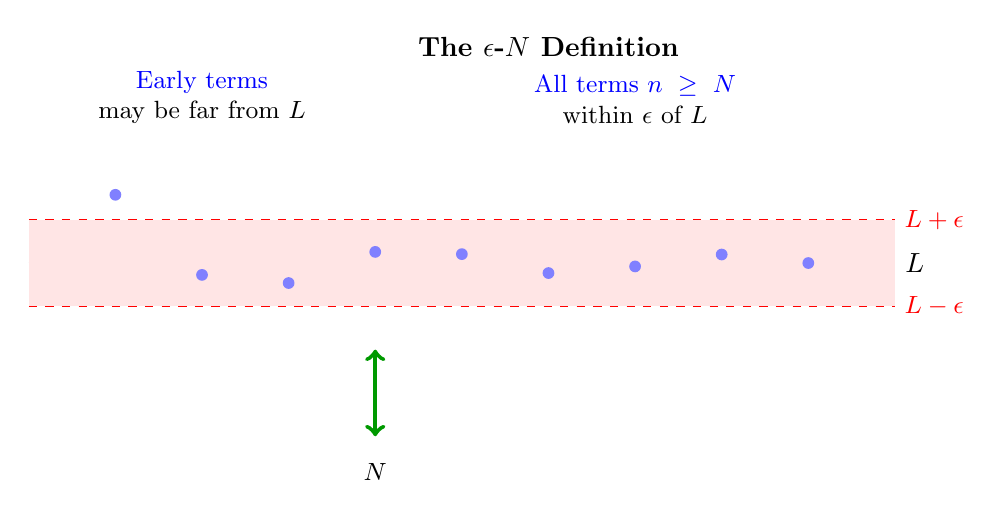
\begin{tikzpicture}[scale=1.1]
    \node at (6, 5) {\textbf{The $\epsilon$-$N$ Definition}};
    
    % The limit L
    \draw[thick] (0, 2.5) -- (10, 2.5) node[right] {$L$};
    
    % Epsilon band
    \draw[dashed, red] (0, 3) -- (10, 3) node[right, font=\small] {$L + \epsilon$};
    \draw[dashed, red] (0, 2) -- (10, 2) node[right, font=\small] {$L - \epsilon$};
    
    \fill[red!10] (0, 2) rectangle (10, 3);
    
    % Sequence terms
    \foreach \n in {1,...,9} {
        \pgfmathsetmacro{\y}{2.5 + 0.8/\n * sin(100*\n)}
        \node[circle, fill=blue!50, inner sep=1.5pt] at (\n, \y) {};
    }
    
    % The threshold N
    \draw[<->, ultra thick, green!60!black] (4, 0.5) -- (4, 1.5);
    \node[below, font=\small] at (4, 0.3) {$N$};
    
    \node[above, text width=4cm, align=center, font=\small] at (2, 4) {
        \textcolor{blue}{Early terms} \\
        may be far from $L$
    };
    
    \node[above, text width=4cm, align=center, font=\small] at (7, 4) {
        \textcolor{blue}{All terms $n \geq N$} \\
        within $\epsilon$ of $L$
    };
\end{tikzpicture}
\end{center}

\begin{example}[Prove $\lim_{n \to \infty} \frac{1}{n} = 0$]
\textbf{Claim}: The sequence $a_n = \frac{1}{n}$ converges to $0$.

\textbf{Proof}: Let $\epsilon > 0$ be given (arbitrary).

We need to find $N$ such that for all $n \geq N$:
\[|a_n - 0| < \epsilon\]

This simplifies to:
\[\frac{1}{n} < \epsilon\]

Equivalently: $n > \frac{1}{\epsilon}$.

\textbf{Choose} $N = \lceil \frac{1}{\epsilon} \rceil + 1$ (smallest integer greater than $\frac{1}{\epsilon}$).

Then for all $n \geq N$:
\[n \geq N > \frac{1}{\epsilon} \implies \frac{1}{n} < \epsilon\]

Therefore $|a_n - 0| < \epsilon$ for all $n \geq N$.

Since $\epsilon$ was arbitrary, $\lim_{n \to \infty} \frac{1}{n} = 0$. $\blacksquare$
\end{example}

\begin{example}[Non-convergent Sequence]
Consider $a_n = (-1)^n$, so the sequence is $(−1, 1, −1, 1, −1, \ldots)$.

\textbf{Claim}: This sequence does not converge.

\textbf{Proof}: Suppose for contradiction that $a_n \to L$ for some $L$.

Choose $\epsilon = \frac{1}{2}$.

Then there exists $N$ such that for all $n \geq N$: $|a_n - L| < \frac{1}{2}$.

Consider two consecutive terms: $a_N = (-1)^N$ and $a_{N+1} = (-1)^{N+1} = -a_N$.

Both satisfy $|a_N - L| < \frac{1}{2}$ and $|a_{N+1} - L| < \frac{1}{2}$.

By triangle inequality:
\[|a_N - a_{N+1}| \leq |a_N - L| + |L - a_{N+1}| < \frac{1}{2} + \frac{1}{2} = 1\]

But $|a_N - a_{N+1}| = |a_N - (-a_N)| = 2|a_N| = 2$, contradicting $2 < 1$.

Therefore no such $L$ exists, and the sequence diverges. $\blacksquare$
\end{example}

\section{Properties of Limits}

\begin{theorem}[Uniqueness of Limits]
If $(a_n)$ converges, its limit is unique.

That is, if $a_n \to L$ and $a_n \to M$, then $L = M$.
\end{theorem}

\begin{proof}
Suppose $a_n \to L$ and $a_n \to M$ with $L \neq M$.

Let $\epsilon = \frac{|L - M|}{3} > 0$.

Since $a_n \to L$, there exists $N_1$ such that for all $n \geq N_1$: $|a_n - L| < \epsilon$.

Since $a_n \to M$, there exists $N_2$ such that for all $n \geq N_2$: $|a_n - M| < \epsilon$.

Let $N = \max(N_1, N_2)$. For $n \geq N$:
\begin{align*}
|L - M| &= |L - a_n + a_n - M| \\
&\leq |L - a_n| + |a_n - M| \quad \text{(triangle inequality)} \\
&< \epsilon + \epsilon = 2\epsilon = \frac{2|L - M|}{3}
\end{align*}

Therefore $|L - M| < \frac{2|L - M|}{3}$, which implies $\frac{|L - M|}{3} < 0$, contradiction.

Therefore $L = M$. $\blacksquare$
\end{proof}

\begin{theorem}[Boundedness of Convergent Sequences]
If $(a_n)$ converges, then $(a_n)$ is bounded.

That is, there exists $M > 0$ such that $|a_n| \leq M$ for all $n$.
\end{theorem}

\begin{proof}
Suppose $a_n \to L$.

Choose $\epsilon = 1$. Then there exists $N$ such that for all $n \geq N$: $|a_n - L| < 1$.

By triangle inequality: $|a_n| = |a_n - L + L| \leq |a_n - L| + |L| < 1 + |L|$.

So for $n \geq N$, we have $|a_n| < 1 + |L|$.

For $n < N$, there are only finitely many terms: $|a_1|, |a_2|, \ldots, |a_{N-1}|$.

Let $M = \max(|a_1|, |a_2|, \ldots, |a_{N-1}|, 1 + |L|)$.

Then $|a_n| \leq M$ for all $n$. $\blacksquare$
\end{proof}

\begin{warning}
The converse is \textbf{false}: A bounded sequence need not converge.

\textbf{Example}: $a_n = (-1)^n$ is bounded ($|a_n| = 1$ for all $n$) but does not converge.
\end{warning}

\begin{theorem}[Algebra of Limits]
If $a_n \to L$ and $b_n \to M$, then:
\begin{enumerate}
    \item $a_n + b_n \to L + M$ (sum rule)
    \item $a_n - b_n \to L - M$ (difference rule)
    \item $a_n \cdot b_n \to L \cdot M$ (product rule)
    \item $\frac{a_n}{b_n} \to \frac{L}{M}$ if $M \neq 0$ and $b_n \neq 0$ for all $n$ (quotient rule)
    \item $ca_n \to cL$ for any constant $c \in \mathbb{R}$ (scalar multiplication)
\end{enumerate}
\end{theorem}

\begin{proof}[Proof of Sum Rule]
Let $\epsilon > 0$ be given.

Since $a_n \to L$, there exists $N_1$ such that for all $n \geq N_1$: $|a_n - L| < \frac{\epsilon}{2}$.

Since $b_n \to M$, there exists $N_2$ such that for all $n \geq N_2$: $|b_n - M| < \frac{\epsilon}{2}$.

Let $N = \max(N_1, N_2)$. For $n \geq N$:
\begin{align*}
|(a_n + b_n) - (L + M)| &= |(a_n - L) + (b_n - M)| \\
&\leq |a_n - L| + |b_n - M| \quad \text{(triangle inequality)} \\
&< \frac{\epsilon}{2} + \frac{\epsilon}{2} = \epsilon
\end{align*}

Therefore $a_n + b_n \to L + M$. $\blacksquare$

The other rules follow similarly (product rule requires using boundedness theorem).
\end{proof}

\begin{example}[Using Algebra of Limits]
Find $\lim_{n \to \infty} \frac{3n^2 + 5n - 7}{2n^2 + n + 1}$.

\textbf{Solution}: Divide numerator and denominator by $n^2$:
\[\frac{3n^2 + 5n - 7}{2n^2 + n + 1} = \frac{3 + \frac{5}{n} - \frac{7}{n^2}}{2 + \frac{1}{n} + \frac{1}{n^2}}\]

Since $\frac{1}{n} \to 0$ and $\frac{1}{n^2} \to 0$:
\begin{align*}
\text{Numerator} &\to 3 + 0 - 0 = 3 \\
\text{Denominator} &\to 2 + 0 + 0 = 2
\end{align*}

By quotient rule:
\[\lim_{n \to \infty} \frac{3n^2 + 5n - 7}{2n^2 + n + 1} = \frac{3}{2}\]
\end{example}

\section{Monotone Sequences and Boundedness}

\begin{definition}[Monotone Sequences]
A sequence $(a_n)$ is:
\begin{itemize}
    \item \textbf{Increasing} if $a_n \leq a_{n+1}$ for all $n$
    \item \textbf{Decreasing} if $a_n \geq a_{n+1}$ for all $n$
    \item \textbf{Strictly increasing} if $a_n < a_{n+1}$ for all $n$
    \item \textbf{Strictly decreasing} if $a_n > a_{n+1}$ for all $n$
    \item \textbf{Monotone} if it is either increasing or decreasing
\end{itemize}
\end{definition}

\begin{theorem}[Monotone Convergence Theorem]\index{monotone convergence theorem}\index{sequence!monotone}\index{convergence!of monotone sequences}
\textbf{(a)} Every bounded increasing sequence converges.

\textbf{(b)} Every bounded decreasing sequence converges.
\end{theorem}

\begin{proof}[Proof of (a)]
Let $(a_n)$ be increasing and bounded above.

Let $A = \{a_n : n \in \mathbb{N}\} \subseteq \mathbb{R}$.

Since $A$ is bounded above and non-empty, by completeness of $\mathbb{R}$, $\sup(A)$ exists.

Let $L = \sup(A)$.

\textbf{Claim}: $a_n \to L$.

Let $\epsilon > 0$ be given.

Since $L - \epsilon < L = \sup(A)$, by definition of supremum, $L - \epsilon$ is not an upper bound of $A$.

Therefore there exists $N$ such that $a_N > L - \epsilon$.

Since $(a_n)$ is increasing, for all $n \geq N$: $a_N \leq a_n \leq L$.

Therefore: $L - \epsilon < a_N \leq a_n \leq L < L + \epsilon$.

So $|a_n - L| < \epsilon$ for all $n \geq N$.

Therefore $a_n \to L = \sup(A)$. $\blacksquare$

The proof of (b) is similar, using $\inf(A)$.
\end{proof}

\begin{keyidea}
\textbf{This theorem is powerful}:

To prove convergence of an increasing sequence, we only need to show it's bounded above---we don't need to find the limit explicitly!

The completeness of $\mathbb{R}$ guarantees the limit exists (it's the supremum).
\end{keyidea}

\begin{example}[Decimal Expansions]
Consider the sequence of decimal approximations to $\sqrt{2}$:
\[a_1 = 1, \quad a_2 = 1.4, \quad a_3 = 1.41, \quad a_4 = 1.414, \quad a_5 = 1.4142, \ldots\]

This sequence is:
\begin{itemize}
    \item Increasing: Each term adds more precision
    \item Bounded above: All terms are $< 2$ (since $(\sqrt{2})^2 = 2 < 4 = 2^2$)
\end{itemize}

By the Monotone Convergence Theorem, $(a_n)$ converges.

The limit is $\sqrt{2}$ (the completeness of $\mathbb{R}$ ensures this limit exists).
\end{example}

\begin{center}
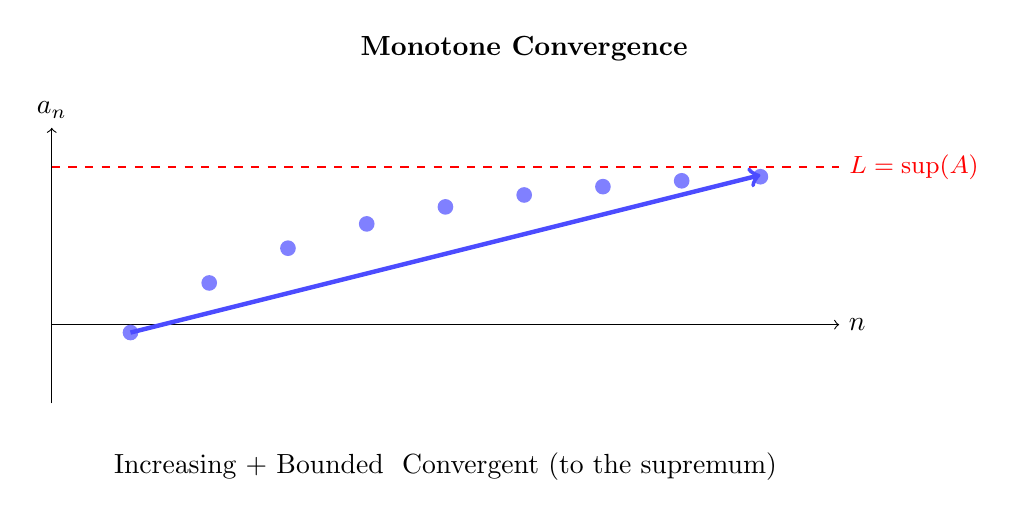
\begin{tikzpicture}[scale=1.0]
    \node at (6, 4.5) {\textbf{Monotone Convergence}};
    
    % Increasing sequence
    \draw[->] (0, 1) -- (10, 1) node[right] {$n$};
    \draw[->] (0, 0) -- (0, 3.5) node[above] {$a_n$};
    
    % The limit
    \draw[dashed, red, thick] (0, 3) -- (10, 3) node[right, font=\small] {$L = \sup(A)$};
    
    % Sequence terms
    \foreach \n in {1,...,9} {
        \pgfmathsetmacro{\y}{3 * (1 - 0.7^\n)}
        \node[circle, fill=blue!50, inner sep=2pt] at (\n, \y) {};
    }
    
    \draw[->, ultra thick, blue!70] (1, 0.9) -- (9, 2.9);
    
    \node[below, text width=10cm, align=center] at (5, -0.5) {
        Increasing + Bounded $\implies$ Convergent (to the supremum)
    };
\end{tikzpicture}
\end{center}

\section{Cauchy Sequences}

\begin{intuition}
To prove $(a_n)$ converges using the $\epsilon$-$N$ definition, we need to know the limit $L$ in advance.

But sometimes we want to know if a sequence converges \textit{without} finding the limit.

\textbf{Cauchy's insight}: A sequence converges if and only if its terms get arbitrarily close \textit{to each other} (not necessarily to a known limit).
\end{intuition}

\begin{definition}[Cauchy Sequence]\index{Cauchy sequence}\index{sequence!Cauchy}\index{completeness!Cauchy criterion}
A sequence $(a_n)$ is \textbf{Cauchy} if:

\[\forall \epsilon > 0, \exists N \in \mathbb{N} \text{ such that } \forall m, n \geq N: |a_m - a_n| < \epsilon\]

Informally: Terms become arbitrarily close to each other as we go far enough in the sequence.
\end{definition}

\begin{keyidea}
\textbf{Convergent vs. Cauchy}:

\textbf{Convergent}: Terms approach a specific limit $L$

\textbf{Cauchy}: Terms approach \textit{each other} (we don't specify what they're approaching)

In $\mathbb{R}$, these are equivalent (due to completeness). In $\mathbb{Q}$, they differ!
\end{keyidea}

\begin{theorem}[Cauchy Criterion]\index{Cauchy criterion}\index{completeness!of real numbers}
A sequence in $\mathbb{R}$ converges if and only if it is Cauchy.
\end{theorem}

\begin{proof}
\textbf{($\Rightarrow$) Convergent implies Cauchy}:

Suppose $a_n \to L$. Let $\epsilon > 0$ be given.

Since $a_n \to L$, there exists $N$ such that for all $n \geq N$: $|a_n - L| < \frac{\epsilon}{2}$.

For $m, n \geq N$:
\begin{align*}
|a_m - a_n| &= |a_m - L + L - a_n| \\
&\leq |a_m - L| + |L - a_n| \\
&< \frac{\epsilon}{2} + \frac{\epsilon}{2} = \epsilon
\end{align*}

Therefore $(a_n)$ is Cauchy. $\checkmark$

\textbf{($\Leftarrow$) Cauchy implies convergent}:

This direction uses completeness of $\mathbb{R}$.

Suppose $(a_n)$ is Cauchy. We show $(a_n)$ is bounded, then construct its limit.

\textit{Step 1: Boundedness}. Choose $\epsilon = 1$. There exists $N$ such that for all $m, n \geq N$: $|a_m - a_n| < 1$.

Fix $n = N$. Then for all $m \geq N$: $|a_m - a_N| < 1$, so $|a_m| \leq |a_N| + 1$.

Let $M = \max(|a_1|, |a_2|, \ldots, |a_{N-1}|, |a_N| + 1)$. Then $|a_n| \leq M$ for all $n$. $\checkmark$

\textit{Step 2: Construct limit}. For each $k \in \mathbb{N}$, let $A_k = \{a_n : n \geq k\}$ (the ``tail'' of the sequence).

Each $A_k$ is bounded and non-empty, so $L_k = \sup(A_k)$ exists by completeness.

The sequence $(L_k)$ is decreasing: $L_1 \geq L_2 \geq L_3 \geq \ldots$ (since $A_1 \supseteq A_2 \supseteq A_3 \supseteq \ldots$).

Also $(L_k)$ is bounded below (by any lower bound of $(a_n)$).

By Monotone Convergence Theorem, $L_k \to L$ for some $L$.

\textit{Step 3: Show $a_n \to L$}. Let $\epsilon > 0$ be given.

Since $(a_n)$ is Cauchy, there exists $N_1$ such that for all $m, n \geq N_1$: $|a_m - a_n| < \frac{\epsilon}{2}$.

Since $L_k \to L$, there exists $N_2$ such that for all $k \geq N_2$: $|L_k - L| < \frac{\epsilon}{2}$.

Let $N = \max(N_1, N_2)$. For $n \geq N$:

Since $L_N = \sup(A_N)$ and $a_n \in A_N$ (because $n \geq N$), we have $a_n \leq L_N$.

Also, by Cauchy property and definition of supremum, $L_N - a_n < \frac{\epsilon}{2}$ (details omitted).

Therefore:
\[|a_n - L| \leq |a_n - L_N| + |L_N - L| < \frac{\epsilon}{2} + \frac{\epsilon}{2} = \epsilon\]

Therefore $a_n \to L$. $\blacksquare$
\end{proof}

\begin{remark}
The direction Cauchy $\Rightarrow$ convergent critically uses completeness of $\mathbb{R}$.

In $\mathbb{Q}$, there exist Cauchy sequences that don't converge (to a rational).

\textbf{Example}: The sequence $1.4, 1.41, 1.414, 1.4142, \ldots$ (rational approximations to $\sqrt{2}$) is Cauchy in $\mathbb{Q}$ but does not converge to any rational number.

This is why we needed to construct $\mathbb{R}$---to complete $\mathbb{Q}$ by adding these missing limits!
\end{remark}

\section{Subsequences and Bolzano-Weierstrass}

\begin{definition}[Subsequence]
Given a sequence $(a_n)$, a \textbf{subsequence} is a sequence $(a_{n_k})$ where $n_1 < n_2 < n_3 < \ldots$ is a strictly increasing sequence of indices.

Informally: Select infinitely many terms from $(a_n)$ in order.
\end{definition}

\begin{example}
From $(1, 2, 3, 4, 5, 6, \ldots)$:
\begin{itemize}
    \item Even terms: $(2, 4, 6, 8, \ldots)$ is the subsequence $(a_{2k})$
    \item Odd terms: $(1, 3, 5, 7, \ldots)$ is the subsequence $(a_{2k-1})$
    \item Powers of 2: $(2, 4, 8, 16, \ldots)$ is the subsequence $(a_{2^k})$
\end{itemize}
\end{example}

\begin{theorem}[Subsequences of Convergent Sequences]
If $a_n \to L$, then every subsequence $(a_{n_k})$ also converges to $L$.
\end{theorem}

\begin{proof}
Let $\epsilon > 0$ be given.

Since $a_n \to L$, there exists $N$ such that for all $n \geq N$: $|a_n - L| < \epsilon$.

Since $n_k$ is strictly increasing and $n_k \geq k$ for all $k$, we have: for $k \geq N$, $n_k \geq k \geq N$.

Therefore $|a_{n_k} - L| < \epsilon$ for all $k \geq N$.

Thus $a_{n_k} \to L$. $\blacksquare$
\end{proof}

\begin{theorem}[Bolzano-Weierstrass Theorem]\index{Bolzano-Weierstrass theorem}\index{sequence!bounded}\index{subsequence!convergent}
Every bounded sequence in $\mathbb{R}$ has a convergent subsequence.
\end{theorem}

\begin{proof}[Proof Sketch]
Let $(a_n)$ be bounded: $|a_n| \leq M$ for all $n$.

The sequence lives in the interval $[-M, M]$.

\textit{Idea}: Repeatedly bisect intervals to find a convergent subsequence.

\textbf{Step 1}: Divide $[-M, M]$ into $[-M, 0]$ and $[0, M]$. At least one half contains infinitely many terms of $(a_n)$. Choose such a half and call it $I_1$.

\textbf{Step 2}: Divide $I_1$ in half. Again, one half contains infinitely many terms. Choose such a half and call it $I_2$.

\textbf{Continue}: Obtain nested intervals $I_1 \supseteq I_2 \supseteq I_3 \supseteq \ldots$ with $\text{length}(I_k) = \frac{2M}{2^k} \to 0$.

Choose $a_{n_1} \in I_1$, $a_{n_2} \in I_2$ with $n_2 > n_1$, $a_{n_3} \in I_3$ with $n_3 > n_2$, etc.

The subsequence $(a_{n_k})$ is Cauchy (since terms are in intervals of shrinking length).

By Cauchy criterion, $(a_{n_k})$ converges. $\blacksquare$
\end{proof}

\begin{keyidea}
Bolzano-Weierstrass is \textbf{powerful}:

Even if a bounded sequence doesn't converge (like $(-1)^n$), we can always extract a convergent subsequence.

This theorem is crucial in proving existence results in analysis.
\end{keyidea}

\section{Series: Infinite Sums}

\begin{intuition}
A \textbf{series} is an ``infinite sum'':
\[\sum_{n=1}^\infty a_n = a_1 + a_2 + a_3 + \cdots\]

But what does this mean rigorously? We can't literally ``add infinitely many things.''

\textbf{Solution}: Define convergence via partial sums.
\end{intuition}

\begin{definition}[Series and Partial Sums]
Given a sequence $(a_n)$, the \textbf{$n$-th partial sum} is:
\[S_n = \sum_{k=1}^n a_k = a_1 + a_2 + \cdots + a_n\]

The \textbf{series} $\sum_{n=1}^\infty a_n$ \textbf{converges} if the sequence of partial sums $(S_n)$ converges.

If $S_n \to S$, we write:
\[\sum_{n=1}^\infty a_n = S\]
and call $S$ the \textbf{sum of the series}.
\end{definition}

\begin{example}[Geometric Series]
Consider $\sum_{n=0}^\infty r^n = 1 + r + r^2 + r^3 + \cdots$ for $|r| < 1$.

The partial sum is:
\[S_n = \sum_{k=0}^n r^k = \frac{1 - r^{n+1}}{1 - r} \quad \text{(geometric sum formula)}\]

As $n \to \infty$:
\[S_n = \frac{1 - r^{n+1}}{1 - r} \to \frac{1}{1 - r} \quad \text{(since $r^{n+1} \to 0$ when $|r| < 1$)}\]

Therefore:
\[\sum_{n=0}^\infty r^n = \frac{1}{1 - r} \quad \text{for } |r| < 1\]

If $|r| \geq 1$, the series diverges.
\end{example}

\begin{example}[Harmonic Series]
The harmonic series is:
\[\sum_{n=1}^\infty \frac{1}{n} = 1 + \frac{1}{2} + \frac{1}{3} + \frac{1}{4} + \cdots\]

\textbf{Claim}: This series diverges (even though $\frac{1}{n} \to 0$).

\textbf{Proof}: Group terms:
\begin{align*}
S_n &= 1 + \frac{1}{2} + \left(\frac{1}{3} + \frac{1}{4}\right) + \left(\frac{1}{5} + \frac{1}{6} + \frac{1}{7} + \frac{1}{8}\right) + \cdots \\
&> 1 + \frac{1}{2} + \left(\frac{1}{4} + \frac{1}{4}\right) + \left(\frac{1}{8} + \frac{1}{8} + \frac{1}{8} + \frac{1}{8}\right) + \cdots \\
&= 1 + \frac{1}{2} + \frac{1}{2} + \frac{1}{2} + \cdots \to \infty
\end{align*}

Therefore $S_n \to \infty$, and the series diverges. $\blacksquare$
\end{example}

\begin{theorem}[Necessary Condition for Convergence]
If $\sum_{n=1}^\infty a_n$ converges, then $a_n \to 0$.
\end{theorem}

\begin{proof}
Suppose $S_n = \sum_{k=1}^n a_k \to S$.

Then:
\[a_n = S_n - S_{n-1} \to S - S = 0\]

Therefore $a_n \to 0$. $\blacksquare$
\end{proof}

\begin{warning}
The converse is \textbf{false}: $a_n \to 0$ does \textbf{not} imply $\sum a_n$ converges.

\textbf{Counterexample}: Harmonic series $\sum \frac{1}{n}$ has $\frac{1}{n} \to 0$ but diverges.
\end{warning}

\section{Looking Forward: Continuity and Calculus}

\begin{intuition}
With sequences and limits mastered, we can now rigorously define:

\textbf{Continuity}: $f$ is continuous at $x$ if $f(x_n) \to f(x)$ whenever $x_n \to x$

\textbf{Derivatives}: $f'(x) = \lim_{h \to 0} \frac{f(x+h) - f(x)}{h}$

\textbf{Integrals}: $\int_a^b f(x) \, dx = \lim_{n \to \infty} \sum_{i=1}^n f(x_i^*) \Delta x$

All of calculus reduces to limits of sequences. We've built the foundation.
\end{intuition}

\begin{center}
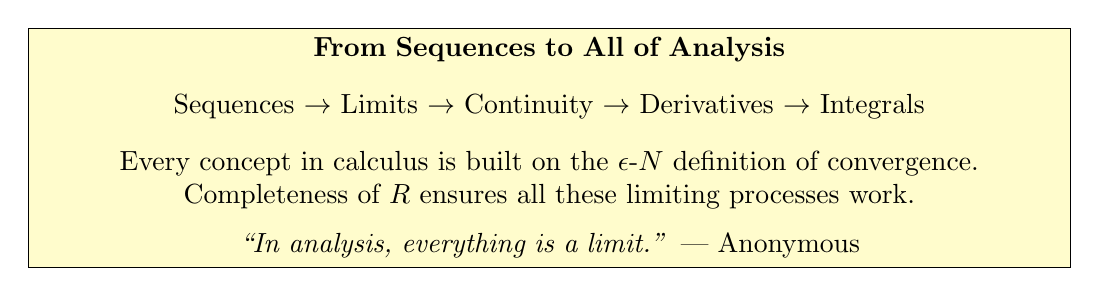
\begin{tikzpicture}[scale=1.0]
    \node[rectangle, draw, fill=yellow!20, text width=13cm, align=center] at (6.5, 0) {
    \textbf{From Sequences to All of Analysis} \\[0.3cm]
    Sequences $\to$ Limits $\to$ Continuity $\to$ Derivatives $\to$ Integrals \\[0.3cm]
    Every concept in calculus is built on the $\epsilon$-$N$ definition of convergence. \\
    Completeness of $\mathbb{R}$ ensures all these limiting processes work. \\[0.2cm]
    \textit{``In analysis, everything is a limit.''} --- Anonymous
    };
\end{tikzpicture}
\end{center}
